Error-resilience is typically a topic discussed orthogonally to congestion
control and the main reason is that, error-resilience caters to handling
packet loss while congestion control caters to the amount of information sent
over the network. This chapter is based on our work on unifying
error-resilience and congestion control.

In \citepub{c:err}, we evaluate the performance of the various
error-resilience schemes available for use in interactive multimedia
communication (mainly applicable to H.264). These are: using Negative
Acknowledgement (NACK) or Packet Loss Indication (PLI), Forward Error
Correction (FEC) or Unequal Level of Protection (ULP), slice size adaption
(SSA), and Reference Pictures Selection Indication (RPSI). We evaluate the
performance of the proposed mechanisms in diverse scenarios in a simulated
environment using real-world 3G loss patterns. Lastly, based on our
observations, we define the applicability of the various error-resilience with
respect to end-to-end delay and packet loss.

In \citepub{c:fecrc}, we propose using FEC not only for error-resilience but
also for congestion control. Instead of probing for available capacity by
increasing the sending rate of the media flow, we propose introducing
redundancy. If a packet gets lost and the added FEC packet arrives in time the
receiving endpoint would recover the lost packet. However, if the packet is
not lost, by introducing the FEC packet the sender not only discovers that
there is additional available capacity, but also has a sense of the magnitude
(at minimum) of the available capacity. We compare our proposal with our
previous work in \citepub{c:3grc} and \citepub{c:hetrc}, and Google's
congestion control~\cite{draft.rrtcc}. We evaluate the performance of the
mechanisms in diverse scenarios implemented in a simulation environment and in
our testbed.

\section{Error-resilience Schemes}
% explain all 4 and the adaptivity

\begin{figure}
\centerline {
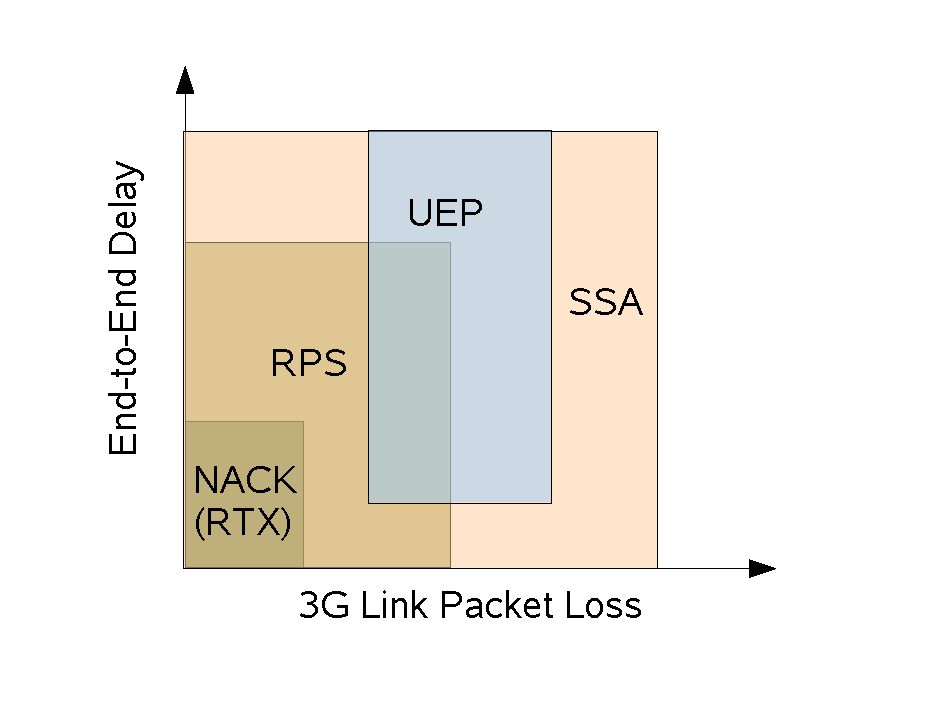
\includegraphics[width=0.9\textwidth]{chap6_apply_err}
}
\caption{Applicability of the error-resilience schemes in heterogeneous
environment containing both wireless and wired links.}
\label{chap6:fig_err}
\end{figure}

\section{Using FEC for Congestion Control}

% Figure with the idea: FEC for CC

% Table of FEC, C-NADU and RRTCC :)